%\begin{savequote}[75mm] 
%Nulla facilisi. In vel sem. Morbi id urna in diam dignissim feugiat. Proin molestie tortor eu velit. Aliquam erat volutpat. Nullam ultrices, diam tempus vulputate egestas, eros pede varius leo.
%\qauthor{Quoteauthor Lastname} 
%\end{savequote}

\chapter{Deep Learning -- Tying Unsupervised and Supervised Learning Together}

\newthought{Formalized, multi-level learning} is the main goal in deep learning -- developing a layered model corresponding to distinct levels of concepts. Deep architectures are composed of multiple levels of non-linear operations, such as in neural nets with many hidden layers or in complicated propositional formulae re-using many sub-formulae\citep{Bengio2009LearningDeep}.

\section{Biological Inspiration}

Trends in Neural Network formalism tend to coincide with changes in our understanding of how the brain works. An \ann{} can be formulated as clusters of neurons which fire via activation functions to produce some desired representation of an input.

In order to thoroughly understand the notion of \dl{} within an \ann{}, I give a linear algebraic formulation, along with a formal description of the training procedure.

\section{A General Neural Network}

More often than not, a $k$-layered\footnote{I consider the input a layer.} \ann{} is thought of as a directed, acyclic $k$-partite graph, with some operator taking a transformed sum of a flow into each node. However, this is not a pragmatic way of formulating a neural network. In lieu of graphs, I use an  linear algebraic formulation. 
%\footnote{I consider the case where our targets are $k$ classes, encoded with 1-versus-all encoding, and we try to classify a vector \mathbf{x} as it is presented}

Formally, consider a dataset $X\in\R^{n\times p}$, where we have $p$ observations. Each observation is a vector $\mathbf{x}\in\R^n$. We also have a set of target values $T\in\R^{k\times p}$, where a target associated with an observation is a vector\footnote{Note that we are predicting $k$ targets.} $\mathbf{t}\in\R^k$.

An \ann{}, given an observation $\mathbf{x}$, tries to predict $\mathbf{t}\in\R^k$. Formally, a neural network $\mathcal{N}$ can be considered as a tuple $\{ C, f, g \}$, where:
\label{nn_conditions}
\begin{enumerate}

\item $f$ is some chosen neural activation function.
\item $g$ is either the identity function or the $\smax(\cdot)$ function.
\item $C$ is a collection of pairs of matrices and vectors ${(A_i, b_i)}_{i=1}^{n}$ such that \eqref{condition on dimensions} and \eqref{condition on product} are satisfied, and $\boxtimes_{C}^{f}(\mathbf{x})\in\R^k$
\end{enumerate}

Given this tuple, the \emph{hypothesis} produced from a neural network $\mathcal{N}$ can be written as

\begin{equation}
\label{net_prediction}
H(\mathbf{x} | \mathcal{N}) = g(\boxtimes_{C}^{f}(\mathbf{x}))
\end{equation}

which leads to a general, rather abstract formulation of the solution of the \ann{}. Let $E : (\mathbf{x}, \mathbf{y}) \longrightarrow \R$ be an error function that maps two vectors in a space to some value\footnote{Common choices include Sum-of-Squared-Errors and Cross-Entropy}. We try to find

\begin{equation}
\label{prob_formulation}
\min_{C} \sum_{(\mathbf{x}, \mathbf{t}) \in (X, T)}E(\mathbf{t}, H(\mathbf{x} | \mathcal{N}))
\end{equation}

which solves our problem of the best neural network given our observed $X$ and $T$. However, this is a purely theoretical formulation -- we must place constraints on how to solve the minimization problem outlined in \eqref{prob_formulation}.


\section{Pragmatism in forming a hypothesis}

How do we choose an activation function, as specified in the conditions for the neural network in \ref{nn_conditions} on page \pageref{nn_conditions}? In practice, the standard sigmoid unit and hyperbolic unit are often use. In this implementation, we will use the standard sigmoidal unit.

Clearly, the formalized prediction from the \nn{} \`{a} la \eqref{net_prediction} is a series of simple \texttt{AXPY} operations which can be easily optimized. Take our \nn{} $\mathcal{N}=\{ C, f, g \}$. From $$H(\mathbf{x} | \mathcal{N}) = g(\boxtimes_{C}^{f}(\mathbf{x}))$$, we can see the following. Suppose we have a \nn{} with $\ell$ layers. We will then have $\ell-1$ matrices and vectors in $C$. Label them $(W_i, b_i)$. We let $\mathbf{a}^{(1)} = \mathbf{x}$,  which allows us to say that 
\begin{eqnarray}
\mathbf{z}^{(i+1)} &=& W_i \mathbf{a}^{(i)} + b_i\\
\mathbf{a}^{(i+1)} &=& 
	\begin{cases} 
		f(\mathbf{z}^{(i+1)}), & \mbox{if } i+1 \neq \ell \\ 
		g(\mathbf{z}^{(i+1)}), & \mbox{otherwise}
	\end{cases}
\end{eqnarray}

Such a formulation lends itself to implementation in any language that can accommodate fast linear algebra.

\section{How can we train a basic \ann{}?}
\label{basix}

Training an \ann{} is done most frequently by so-called \emph{backpropagation}. Backpropagation proves itself useful in the training of both basic and Deep \nn{}s. In this section, we discuss -- in detail -- the implementation of backpropagation using efficient linear algebra.

We can break backpropagation into two parts --  the \emph{feed-forward step} step and \emph{backpropagation of errors}. Essentially, we use the structure of the neural network to define a gradient of cost function associated with the prediction errors that the network produces. 

More formally, suppose we have a collection of data points (column vectors) $\{\mathbf{x}_i\}_{i=1}^n$, where we have that $\mathbf{x}_i\in\R^k$. We can now define our objective function in a more concrete fashion than equation \eqref{prob_formulation}. We here consider the case of multi-class classification -- an instance in which the literature suggests the use of a $\log_2$ cross-entropy function. The derivation of gradients with respect to other error functions follows a similar form, and is omitted here for the sake of brevity. For an individual observation $\mathbf{x}\in\R^k$, a neural network $\mathcal{N}$, the predicted posteriors $\mathbf{p} = \smax(\boxtimes_{C}^{s}(\mathbf{x}))$, and a target vector of one-versus-all class encoding $\mathbf{t}\in\R^p$, we have an error of 
\begin{equation}
\Phi(\mathbf{x}, \mathbf{t}, \mathcal{N}) = -\text{sum}(\log_2(\mathbf{p}) \odot \mathbf{t}).
\end{equation}

To correct the errors our model produces with the posterior vector $\mathbf{p}$, we take a derivative of $\Phi$ with respect to $\mathbf{p}$. We have that 
\begin{equation}
\label{eq:ce_error}
\frac{\partial\Phi}{\partial\mathbf{p}} = -\mathbf{t} \oslash \log(2)\mathbf{p}
\end{equation}

Notice above that only one element of $\mathbf{t}$, call it $t_i$, will be equal to one, and the rest will be zero, since we use one-versus-all class encoding. Now, notice that if the $p_i$ corresponding to $t_i$ is small, then that element of the gradient will blow up, correcting the mistake that the model made. 

We proceed layer by layer. The prediction can be written as $\mathbf{p} = g(\mathbf{z}^{(\ell-1)})$. For the final layer $\ell$ of the network, define

\begin{eqnarray}
\label{eq:finallayer}
\xi^{(\ell)} &=& -(\mathbf{t} \oslash \log(2)\mathbf{p}) \odot g'(\mathbf{z}^{(\ell-1)})\\
 &=& - (\mathbf{t} \oslash \log(2) \mathbf{p}) \odot g(\mathbf{z}^{(\ell-1)}) \odot (\mathbf{1} - g(\mathbf{z}^{(\ell-1)}))\\
 &=& -(\mathbf{t} \oslash \log(2)\mathbf{p}) \odot \mathbf{p} \odot (\mathbf{1} - \mathbf{p})\\
 &=& -\frac{1}{\log(2)}(\mathbf{1} - \mathbf{p}).
\end{eqnarray}

We can the design a similar quantity for each layer below the output layer. Taking derivatives, we have that, for each $i< \ell$,

\begin{equation}
\label{update1}
\xi^{(i)} = (W_i^T\xi^{(i+1)})\odot f\:'(\mathbf{z}^{(i)})
\end{equation}

Using these quantities, we can now find recursive definitions for derivatives with respect to our cost function. We have that 
\begin{eqnarray}
\label{eq:gradients}
\frac{\partial\Phi}{\partial W_i} &=& \xi^{(i+1)}(\mathbf{a}^{(i)})^T\\
\frac{\partial\Phi}{\partial \mathbf{b}^{(i)}} &=& \xi^{(i+1)}.
\end{eqnarray}
Notice that depending on whether or not we use a network for classification or regression, the only quantity that will change in this derivation is $\xi^{(\ell)}$ in equation \eqref{eq:finallayer}. Using equation \eqref{eq:gradients}, we can now write update rules for our optimization procedure. Note that for this derivation, we use pure online updates -- that is, we make adjustments to the gradient after each new labelled example. The basic update becomes then becomes
\begin{equation}
\theta \longleftarrow \theta - \gamma \Deriv{\Phi}{\theta},
\end{equation}
for each $\theta\in(W_i, \mathbf{b}_i)\in C$, and for some small, user-determined \emph{learning parameter} $\gamma$.

\subsection{Gaining Momentum}

In practice, it is well known that a simple gradient update is subject to noise and can suffer from the "ping pong" effect, moving around the local optimal solution without converging quickly. To ameliorate this problem, we utilize \emph{momentum}, which allows us to dampen sharp changes in gradient 
updates. Intuitively, momentum uses a running weighted average of updates to ensure that the gradient update is more resistant to noise in clearly noisy nature of the cost function. 

Formally, if we consider time steps $t$, we have that for a momentum parameter $\mu\in[0,1)$, our update rule becomes 
\begin{eqnarray}
\label{eq:updaterule}
\Delta\theta_{t} &=& (\mu - 1)\gamma\Deriv{\Phi}{\theta_t} + \mu\Delta\theta_{t - 1}\\
\theta_{t+1} &=& \theta_t + \Delta\theta_{t},
\end{eqnarray}
for each $\theta\in(W_i, \mathbf{b}_i)\in C$ which dampens out fluctuations in changes to the gradient.



\section{Extracting Features using \ann{}s}

\subsection{The Basic Autoencoder}

We now shift our attention to \ann{}s that serve as unsupervised learning algorithms. Using \ann{}s, we can learn a new representation of our original data in a new feature space. The process  consists of two steps -- an encoding step, and a decoding step. Such \ann{} is called an \emph{autencoder}. We learn a non-linear \emph{encoding} that can then be linearly \emph{decoded} to recover the original dataset. Obtaining a reliable non-linearly extracted lower dimensional representation is extremely valuable. Intuitively, we train our neural network to estimate an approximation of the identity function. We now provide a simple formulation of such an idea.

Formally, consider the following. Consider our \emph{unlabelled} dataset$\{\mathbf{x}_i\}_{i=1}^n$, where we have that $\mathbf{x}_i\in\R^k$. Suppose we want to map each $\mathbf{x}_i$ to a new vector $\mathbf{y}\in\R^p$ with $p < k$. We wish to find two matrices -- $A\in\R^{p\times k}, B\in\R^{k\times p}$ -- and two vectors  $\mathbf{a}\in\R^p, \mathbf{b}\in\R^k$, that form good encoder-decoder pair as follows. For any $i$, the encoded features of $\mathbf{x}_i$ are represented by the vector 
\begin{equation}
\mathbf{f}_i = s(A\mathbf{x}_i + a)
\end{equation} 
which is clearly in $\R^p$. We now have that our reconstructed input is 
\begin{equation}
\tilde{\mathbf{x}}_i = B\mathbf{f}_i+b
\end{equation}

To solve this problem, i.e., to have $\tilde{\mathbf{x}}_i$ be similar to $\mathbf{x}_i$, we formulate this as an optimization problem. Our problem now becomes
\begin{equation}
\label{encodeobj}
\min_{A, B, \mathbf{a},\mathbf{b}} \frac{1}{2}\sumn{i} \Vert \mathbf{x}_i - \tilde{\mathbf{x}}_i \Vert ^ 2
\end{equation}

Clearly, we cannot find an analytical solution to this problem -- however, we can use gradient descent to to find our encoder pair $(A,\mathbf{a})$ and decoder $(B, \mathbf{b})$. Similarly to Section \ref{basix}, we can derive gradients of Equation \eqref{encodeobj}. We can re-write Equation \eqref{encodeobj} as 

\begin{equation}
\min_{A,B,a,b} \rho(A,B,a,b)
\end{equation}

where 
\begin{equation}
\label{eqrho}
\rho(A,B,a,b) = \frac{1}{2}\sumn{i} \Vert \mathbf{x}_i -  (B [s(A\mathbf{x}_i + a)]+b) \Vert ^ 2
\end{equation}

By taking matrix derivatives, we then have that, for a given observation $\mathbf{x}_i$,

\begin{eqnarray}
\label{grads_of_auto}
\Deriv{\rho}{B}&=& -(\mathbf{x}_i -\tilde{\mathbf{x}}_i) \mathbf{f}_i^T \\ 
\Deriv{\rho}{b}&=& -(\mathbf{x}_i - \tilde{\mathbf{x}}_i) \\
\Deriv{\rho}{A}&=& -B^T(\mathbf{x}_i -\tilde{\mathbf{x}}_i) \odot s'(\mathbf{f}_i)\mathbf{x}_i^T \\
\Deriv{\rho}{a}&=& -B^T(\mathbf{x}_i -\tilde{\mathbf{x}}_i) \odot s'(\mathbf{f}_i)
\end{eqnarray}

which allows us to use a gradient update step of
\begin{equation}
\theta \longleftarrow \theta - \gamma \Deriv{\rho}{\theta}
\end{equation}
for each matrix $\theta\in\{A, B, a, b\}$ and some small learning rate $\gamma$.

\subsection{Stacking and Robust Knowledge}
The basic Autoencoder performs well, but can be improved upon. It is desirable to have such an encoder-decoder pair to be resistant to inherent noise in the training data. Thus, in practice, we perturb the inputs to the Autoencoder, and attempt to have the reconstruction reproduce a original, un-noisy version from the perturbed observation. Formally, for any vector $\textbf{x}\in\R^{k}$ we present, let $\delta\mathbf{x}\sim N(\mathbf{0}_k, \varepsilon^2 I)$, where $\mathbf{0}_k$ is the $k$ dimensional vector of zeros, and $\varepsilon$ is some adequately small scalar value. Now, our reconstructed vector of $\tilde{\mathbf{x}}$ of our input $\mathbf{x}$ will be 

\begin{equation}
\label{denoising}
\tilde{\mathbf{x}} = B[s(A(\mathbf{x} + \delta\mathbf{x}) + \mathbf{a})] + \mathbf{b}
\end{equation}

In this case the gradient update steps in \ref{grads_of_auto} do not change. We still find the gradient with respect to the error when compared to the unperturbed observation. This process, though though not provable, creates a resistance to noise, making the features learned by the autoencoder more resistant to noise. Thus, we refer to equation \eqref{denoising} as a Denoising Autoencoder. As new, previously unseen examples are presented, we assume that they have noise associated with them, and are presented as-is --i.e., no perturbation -- to the encoder. In addition to creating more robust features, such a procedure makes the risk of overtraining much lower.

Take any trained denoising autoencoder with parameters $(A,B,a,b)$ that maps vectors $\mathbf{x}\in\R^k$ to features $\mathbf{f}\in\R^{p}$, with $p<k$. Define the function

\begin{equation}
\label{featuremapping}
\mathcal{F}_{(A,a)}^{k\rightarrow p}(\mathbf{x}) = s(A(\mathbf{x}) + \mathbf{a})
\end{equation}

which is syntactical sugar around the encoding step, which involves the encoding pair $(A,a)$. Suppose we wished to develop more abstract features. Using equation \eqref{featuremapping}, we can develop a collection of increasing \emph{abstract} autoencoders -- that is, autoencoders that develop progressively more abstract representations of the dataset. 

Formally, suppose we start from a dataset of dimension $p = d_0$, and we wish to map -- iteratively --  to each $\d_i\in\{d_i\}_{i=1}^{\ell}$, that is we map to $d_1$ dimensions, then to $d_2$ dimensions, et cetera. In addition, suppose we have a training set $\{\mathbf{x}_j\}_{j=1}^n$. For each $i\in\{1,\ldots,\ell\}$, let


\begin{equation}
\begin{aligned}
\label{auto_soln}
& (A_i,B_i,a_i,b_i) = \underset{(A,B,a,b)}{\text{argmin}}
& & \frac{1}{2}\sumn{j} \Vert \mathbf{f}_j^{i-1} -  (B[s(A(\mathbf{f}_j^{i-1}+\delta\mathbf{f}_j^{i-1}) + a)]+b) \Vert ^ 2 \\
& \text{subject to}
& & A_i\in\R^{d_i\times d_{i-1}}, a_i\in\R^{d_{i-1}}, B_i\in\R^{d_{i-1}\times d_{i}}, a_i\in\R^{d_{i}} \\
& \text{where}
& & \mathbf{f}^{i}_j = 
	\begin{cases} 
		\mathcal{F}_{(A_{i},a_{i})}^{d_{i-1}\rightarrow d_i}(\mathbf{f}_j^{i-1}), & \mbox{if } i>0\\ 
		\mathbf{x}_j, & \mbox{otherwise}
	\end{cases}
\end{aligned}
\end{equation}


We now have that for each layer $i$, $(A_i,B_i,a_i,b_i)$ is a Denoising Autoencoder. Equation \eqref{auto_soln} provides us with a formalization of greedy, layer-wise training presented in \citep{Vincent:2010fk}. We can greedily start from the first layer, and then train each following layer on the features extracted from the previous layer.




\section{Deep Neural Network Architecture}

Theoretically, there is no reason to have an upper limit on the size of a \nn{}. Adding additional layers to \nn{}s broadens the classes of functions that are representable. However, in practice, we see a phenomenon called a \emph{vanishing gradient}. We (empirically) see that gradients in layers that are farther away from the target values tend towards zero \citep{trainingdifficulty}. This only becomes a problem when we consider how our network is initiated. Since we originally initiate all values in the network to some range $[-a,a]$, we run an increasing risk of any layer being trapped in a local minimum with smaller gradients. Thus, for less abstract layers, the local minima we find are very dependent upon the initial placed on the weights. 

\subsection{Uncovering Features}

Clearly, a deeper \nn{} makes for more potential to generalize to unseen examples. However, such a complicated model makes for difficult tuning and adjustment of the weight matrices $W_i$. How can we help a complicated model learn such a deep representation of a system?

Searching the parameter space of deep neural networks is difficult and not well defined because the training criterion is non-convex and involves many local minima. This was very clearly elaborated upon in   \citep{Erhan:2009}, who showed that with hundreds of completely random initializations, gradient descent -- the standard backpropagation algorithm -- converged to a different local minimum each time, with solutions obtained from random initialization and purely supervised training consistently getting worse for architectures with more than 2 or 3 levels.

We follow the example of \citep{Bengio:2007uq} and \citep{Vincent:2010fk}, who use the autoencoders outlined in Equation \eqref{auto_soln} to initialize the weights of the network before training using labelled examples. The intuition is as follows. The autoencoder training procedure is resistant to the vanishing gradient problem because of a key insight from \citep{Hinton:2006vn}. Instead of training the model whole, we use a \emph{greedy} autoencoder training system similar to equation \eqref{auto_soln} -- proceeding layer by layer, and ensuring each layer forms a feature representation of the input.

More formally, for an input $x$ and a target $t$, a series of Stacked Autoencoders learns the distribution of the input, i.e., $P(x)$. When we learn the distribution $P(x)$, since $P(t\vert x)$ is structurally similar to $P(x)$ \citep{Erhan:2010:WUP:1756006.1756025}, we are able to use this information to learn a better classifier. 

Once we learn the more abstract features using the stacked, deep architecture, we can then use the target values to fine-tune \citep{Hinton:2006vn} all weights in the architecture to map to our target values. The process can be visualized using Figure \ref{fig:deeplearning}, which shows (in green) the denoising pre-training procedure, and the (in blue) fine-tuning procedure used to map the learned feature representation to the target values. Such a procedure in essence acts as a regularizer \citep{Bengio2009LearningDeep}, initializing weights in weight space while pushing towards local minima that represent $P(x)$ well.


\begin{FPfigure} 
\begin{center} 
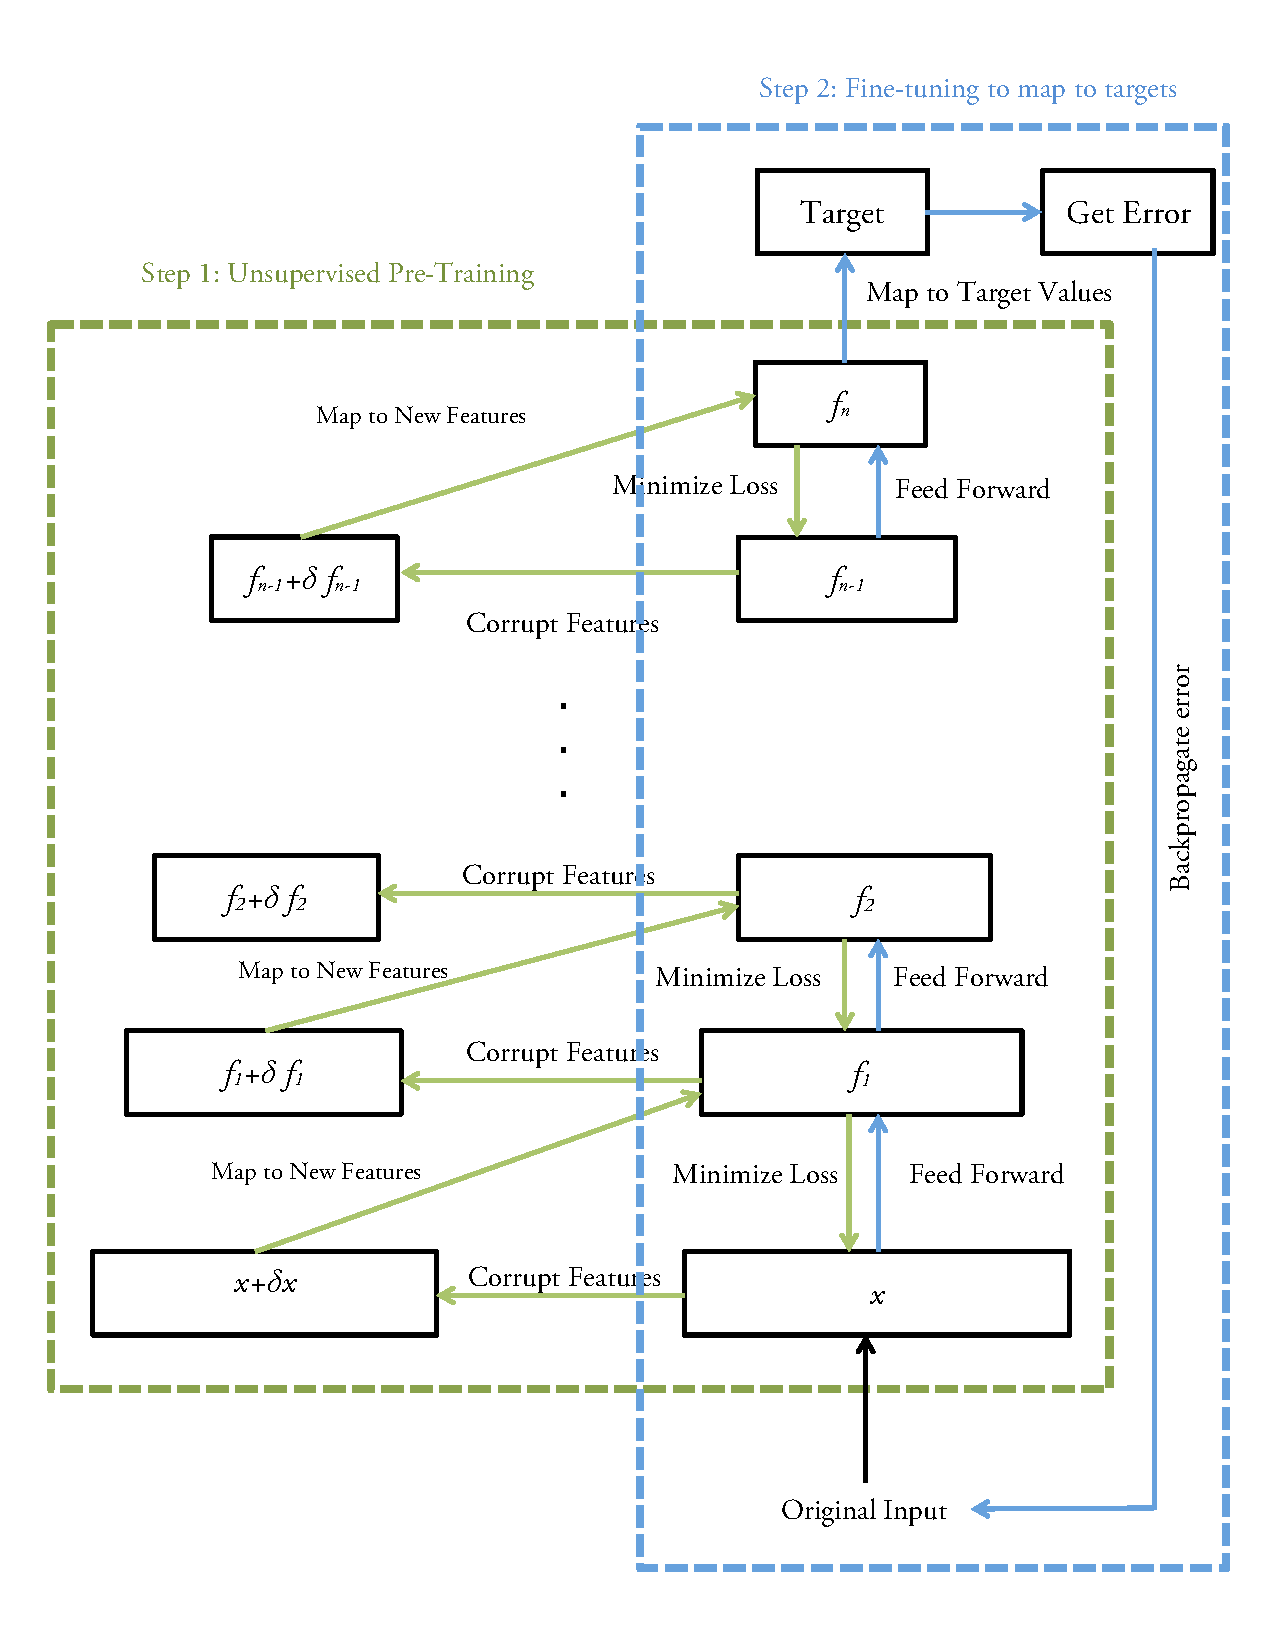
\includegraphics[width=1.2\textwidth]{figures/deeplearning.pdf}
\caption[Short figure name.]{A visualization of the two step Deep Learning process using stacked, denoising autoencoders as feature learners. \label{fig:deeplearning}}
\end{center}
\end{FPfigure}
\afterpage{\clearpage}

\section{Inverting the Problem}

We now turn to the main algorithmic contribution of this thesis, Inverted Deep Network Encoding (IDNE). Once again a sequential process, this idea builds on the notion of fine-tuning, and uses fine tuning to create a better feature representation of the dataset encoded within the deep architecture. 

\section{Choosing What to Learn, or Learning what isn't there}

Clearly, the features we learn through this pre-training procedure are very dependent upon the training sample. That is, proportions of different characteristics within the dataset will change what features are learned within the model. Normally, this is not a problem, as the labelled training data is most likely an accurate, representative sample of the data that a classifier will be predicting over. However, this is not the case with the application of deep learning architectures to particle identification -- in particular, bottom and charm jet tagging. The reason for this is simple twofold -- there is no way to label \emph{real} data, and we cannot fit to kinematics. 

Data that is actually collected from the detector during a run cannot actually be labelled, so any classifier or predictive method must use \emph{Monte Carlo Generated Data}. Physicists understand the Standard Model of Particle Physics well enough to model particle collisions within the ATLAS detector to a very high degree of accuracy. Classifiers are thus trained on Monte Carlo data, which can clearly be labelled, and are then applied to "real" data from the detector. Normally, this is perfect for an algorithm -- seemingly unlimited training data. However, the Monte Carlo Generated data are not modeled perfectly, as there are some parameters in the Standard Model which are approximated under assumptions which may or may not be true. Thus, using \emph{denoising} autoencoders helps to reduce the dependence on the actual values presented to the network, and learns a less Monte Carlo dependent feature representation of the dataset.

In addition to issues with Monte Carlo, we risk overfitting to specific $p_T$ and $\eta$ ranges of the jets we train over. Consider Figure \ref{fig:pT}. We can see that lower $p_T$ ranges are predominantly light jets, which means that any algorithm that tries to minimize error will call anything below a certain $p_T$ a light jet. This does maximize accuracy, as light jets will be the majority of most samples. However, as previously mentioned, we care about being able to identify particles across the $p_T$ spectrum. This begs the question -- is the discrepancy seen at the top of Figure \ref{fig:pT} caused by a disproportionate number of light jets in the entire sample? To answer this, consider the histogram at the bottom of Figure \ref{fig:pT}, which shows the weighted histograms -- i.e., histograms weighted so each flavor has an equal representation. Figure \ref{fig:eta} shows this same phenomenon for $\eta$ -- jets with a high $\vert\eta\vert$ tend to be light jets while jets with a lower $\vert\eta\vert$ tend to be bottom and charm jets. 

\begin{figure}
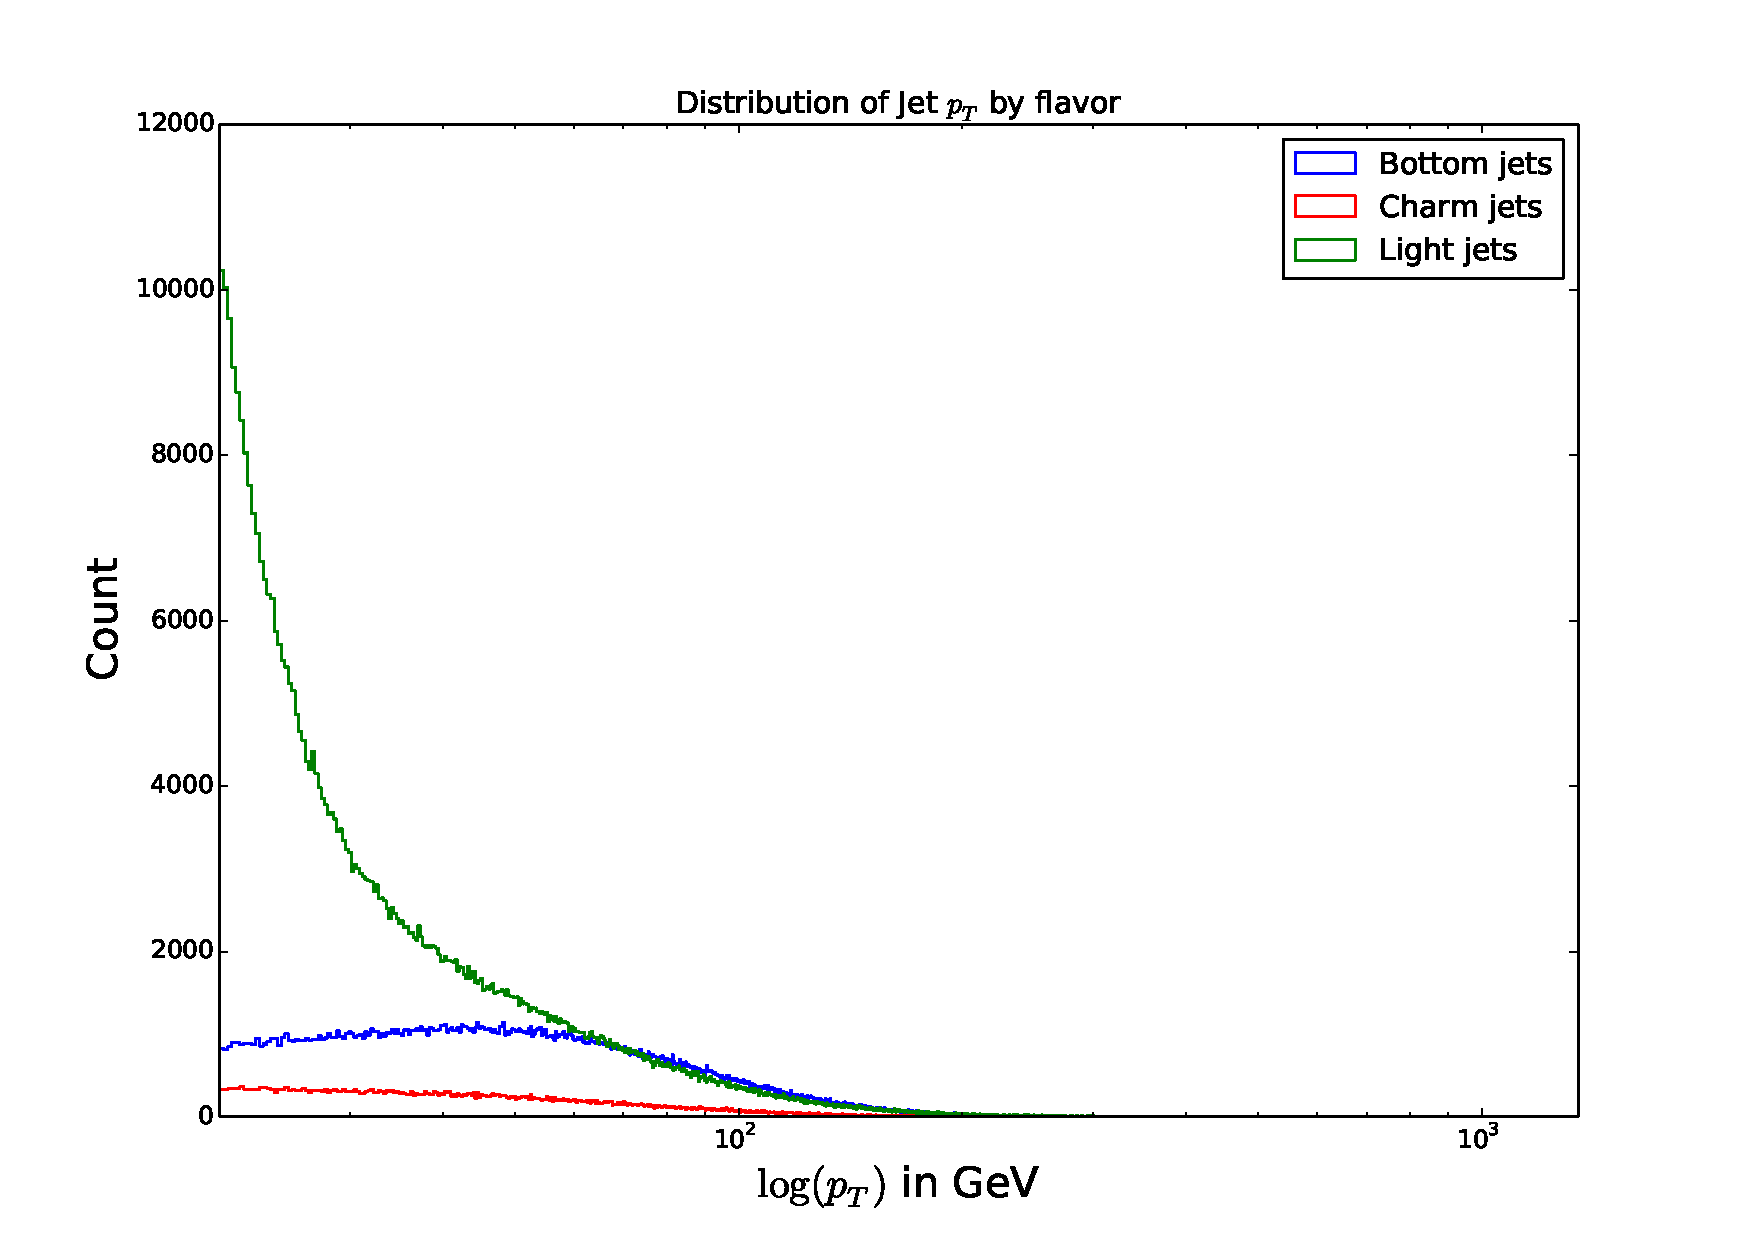
\includegraphics[width=\textwidth]{figures/unweightedpTdistro.pdf}\\
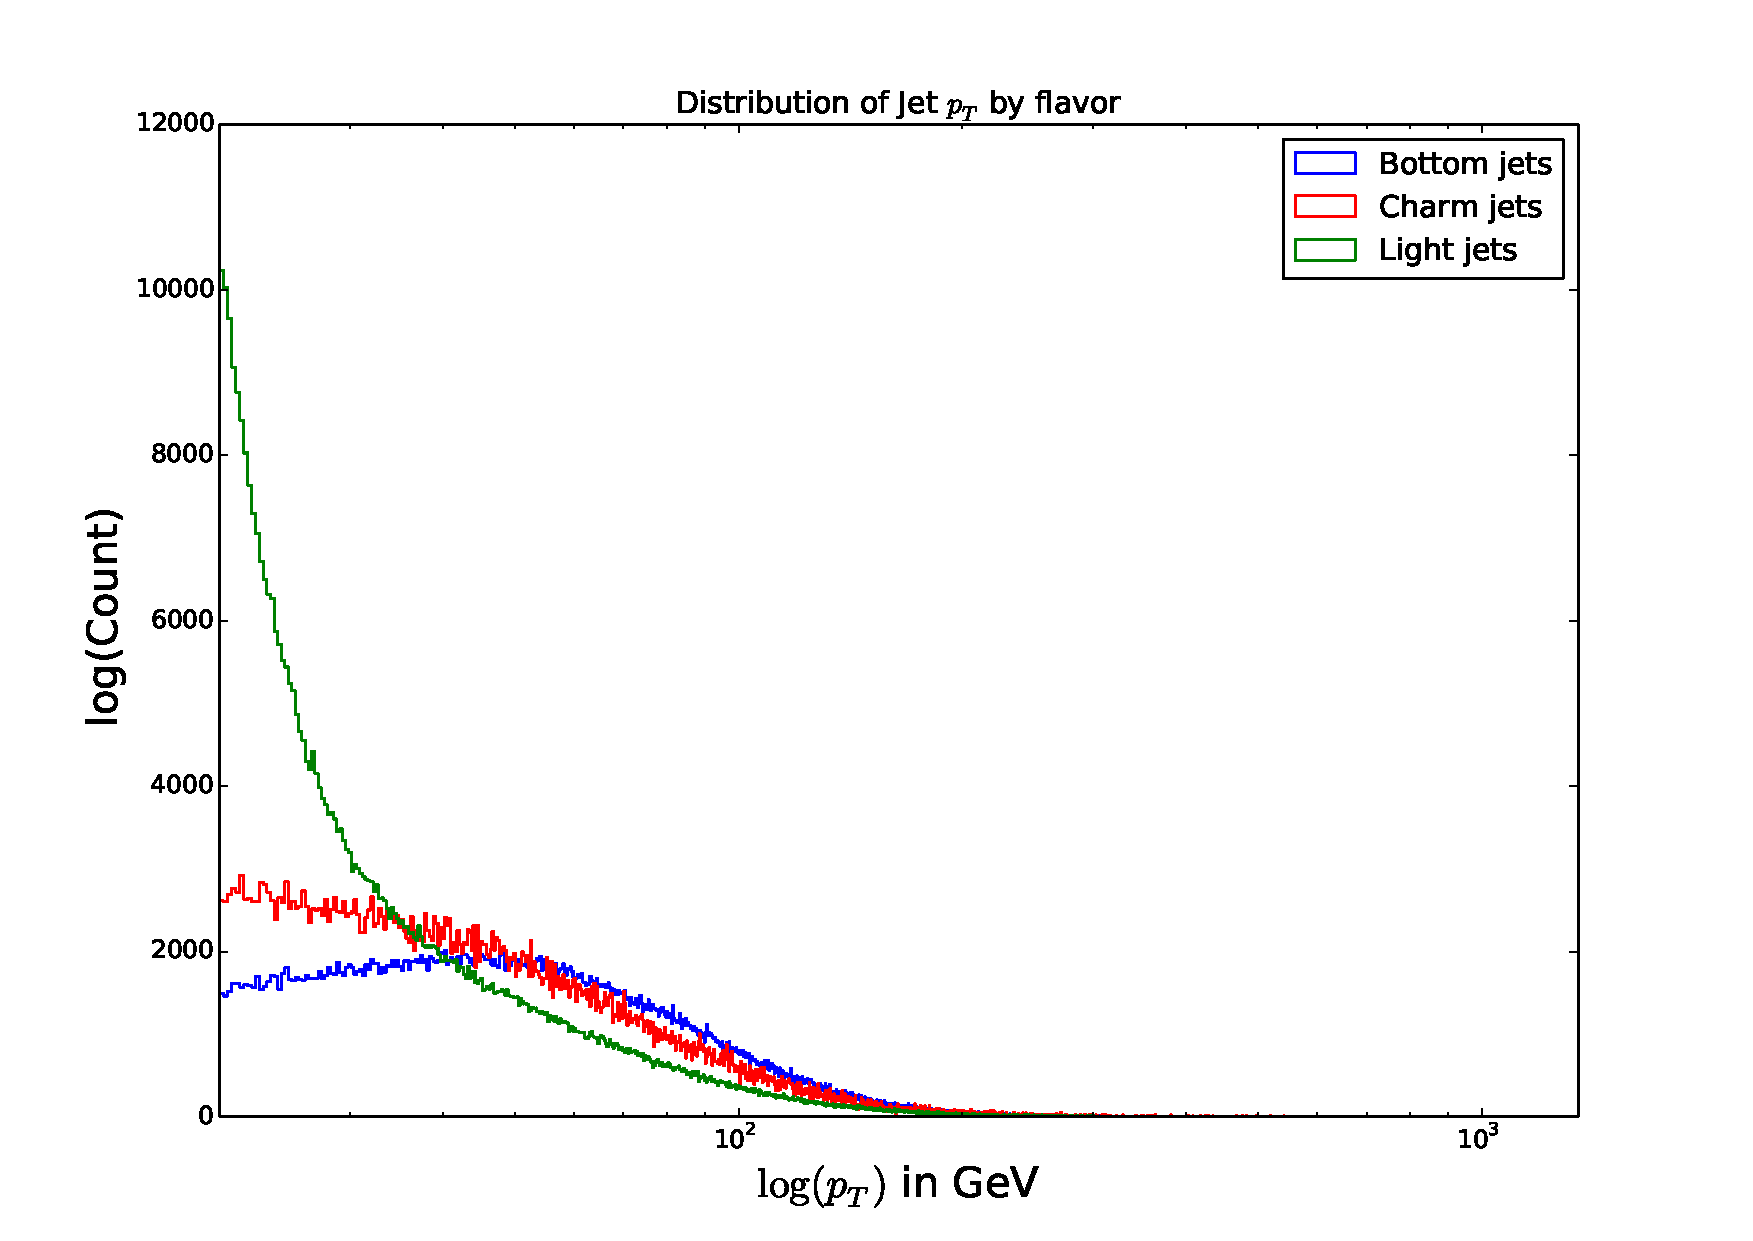
\includegraphics[width=\textwidth]{figures/weightedpTdistro.pdf}
\caption[The ATLAS detector]{Unweighted (Top) and Weighted (Bottom) distributions of Jet $p_T$.
\label{fig:pT}}
\end{figure}
\begin{figure}
\includegraphics[width=\textwidth]{figures/unweightedetadistro.pdf}\\
\includegraphics[width=\textwidth]{figures/weightedetadistro.pdf}
\caption[The ATLAS detector]{Unweighted (Top) and Weighted (Bottom) distributions of Jet $p_T$.
\label{fig:eta}}
\end{figure}


How do we ameliorate this problem? We introduce \emph{online physics reweighting}, which serves to even our the influence of these distributions we see. In essence, we re-weight individual jets order to \emph{flatten} the $p_T$ and $\eta$ distributions across jet type. 

We do the following. Let $f(p_T,\eta \vert \theta)$ be the distribution over $p_T$ and $\eta$ with respect to a certain flavor theta, where $$\sum_\theta \iint\limits_{\R^2}f(p_T,\eta | \theta) = 1.$$ To create a reweighting, we use partitions over the supports of $p_T$ and $\eta$. 

Concretely suppose we want to re-weight a bottom jet that has $p_T$ between the partition values $m_1$ and $m_2$, and $\eta$ between the partition values $e_1$ and $e_2$. Then the weight of the jet with respect to a light majority -- $\omega_u(p_T, \eta, b)$ -- is 
\begin{equation}
\omega_u(p_T, \eta, b) = \frac{\int_{x = m_1}^{m_2}\int_{y = e_1}^{e_2} f(x,y,u)dydx}{\int_{x = m_1}^{m_2}\int_{y = e_1}^{e_2} f(x,y,b)dydx}.
\end{equation}

We do this process over each jet for a user-set partition on $p_T$ and $\eta$, obtaining a $\omega_u(p_T, \eta, \theta)$ for each jet. We define $\omega_u(p_T, \eta, u) = 1$, as we use light jets as our reference distribution. Since we use complete online learning during the optimization procedure, our update rule during optimization from Equation \eqref{eq:updaterule} now becomes -- for a jet of flavor $\theta$ with $p_T$ and $\eta$ -- 

\begin{eqnarray}
\Delta\upsilon_{t} &=& (\mu - 1)\gamma\omega_u(p_T, \eta, \theta)\Deriv{\Phi}{\upsilon_t}+ \mu\Delta\upsilon_{t - 1}\\
\upsilon_{t+1} &=& \upsilon_t + \Delta\upsilon_{t},
\end{eqnarray}
for each $\upsilon\in(W_i, \mathbf{b}_i)\in C$ - the collection of weight matrices of our neural network. 

In addition to this weighting of the gradient, In addition, with a probability $p$. we also add a small amount of noise to the input during supervised training to add robustness. This, when coupled with the reweighting of samples, lets the model learn a sample that is reweighted to have identical $p_T$ and $\eta$ distributions across flavors. The level to which the distributions are the same is controlled by the user set fineness of the partitions of $p_T$ and $\eta$.













